La fibra óptica permite transmitir información a largas distancias mediante luz. Generalmente se usa en cables cables, como los que se colocan en el subsuelo o el suelo marino para el internet.

\begin{figure}[H]
  \centering
  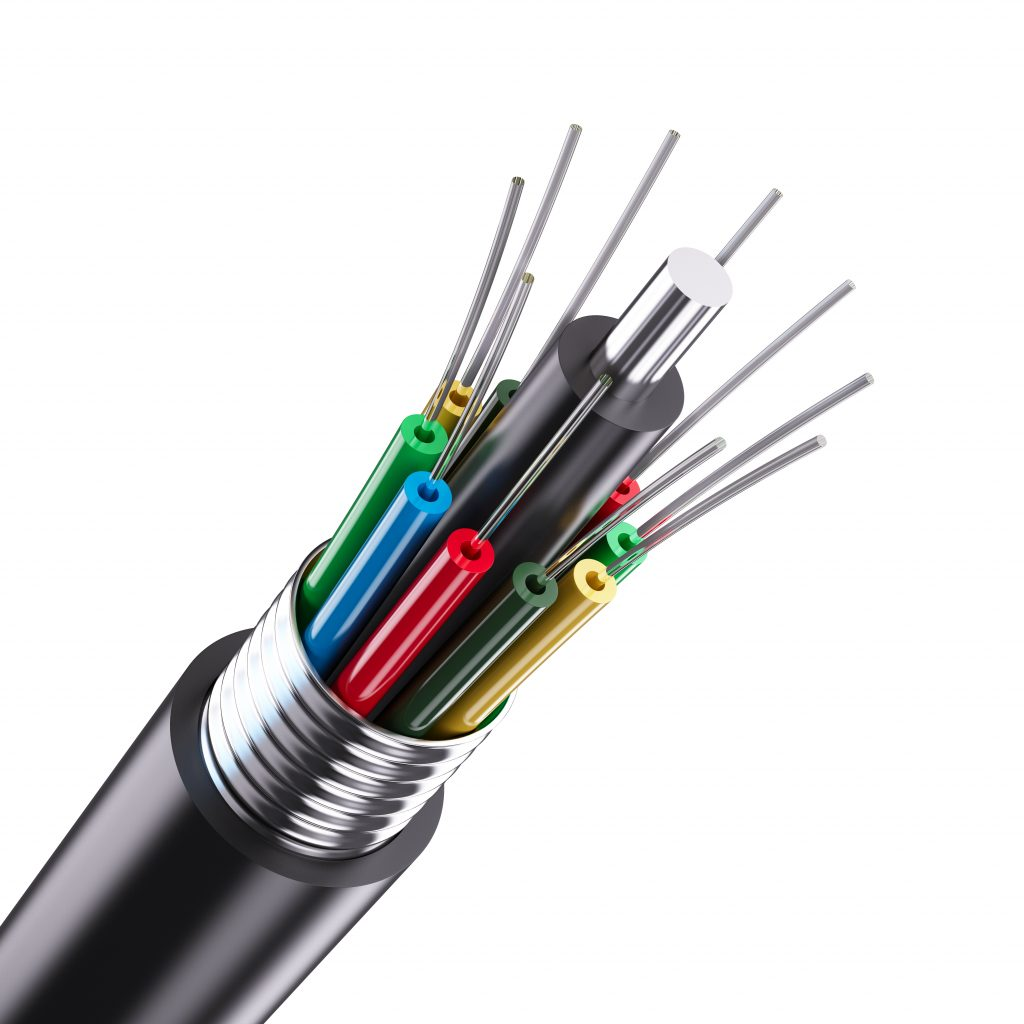
\includegraphics[scale=0.3]{imagenes/fibra_optica.png}
  \caption{Cabe de fibra óptica\cite{nmcfibopt}}
\end{figure}

\subsection{Componentes principales}

Los cables se componen de tres capas principales:

\textbf{Núcleo:} filamento delgado transparente hecho de cristal o plástico.

\textbf{Revestimiento:} rodea al núcleo. También está hecho de cristal o plástico, pero con un índice de refracción diferente del núcleo.

\textbf{Cubierta protectora:} capa exterior que protege el cable de daño físico y ambiental. Puede estar hecho de plástico, kevlar o acero.

\subsection{Procedimiento}

Empieza por convertir datos digitales (texto, imagenes o videos) en señales binarias de luz, utilizando dispositivos como LEDs o láseres.

Los LEDs son más baratos y son usadas en aplicaciones de corto alcance, como LAN (\textit{Local Area Network}). Los láseres, dado su mayor concentrado y poderoso rayo de luz, son ideales para largas distancias y mayor velocidad, como en cables submarinos.

Estas señales son enviadas al cable de fibra óptica, donde viajan a través del núcleo rebotando del revestimiento mediante \reftotint. Una vez las señales de luz alcanzan su destino, son convertidas de vuelta a señales eléctricas por un recividor y enviadas a un dispositivo o red.

Al viajar largas distancias ocurre una pérdida de energía gradual, llamada atenuación. Para reforzar la señal a lo largo del cable se utiliza un repetidor o un amplificador. Los amplificadores con más utilizados que los repetidores\cite{vnfoc}.

\subsection{Ventajas}

Los cables de fibra óptica tienen ventajas clave sobre cables de cobre tradicionales, haciéndolos la opción preferida para redes de comunicación modernas.

\textbf{Mayor ancho de banda y tasa de transferencia:} esto permite mayor velocidad de internet y comunicaciones más eficientes.

\textbf{Inmunidad a interferencia electromagnética:} asegura una conexión más confiable y estable.

\textbf{Reduce la atenuación de la señal:} experimentan menos perdida de señal, en comparación con cables de cobre, lo cual permite una transmisión eficiente de datos sobre largas distancias.

\textbf{Cables más delgados y ligeros:} esto hace que sean más fáciles de instalar y reduce el costo en infraestructura.

\textbf{Mejor seguridad:} puesto que no emiten señales eléctricas son menos suceptibles de pérdidas e intercepciones.
